\subsection{Étude de la variable petalLength}
\subsubsection*{Première approche : graphique}

\vspace{.2cm}

\noindent
\textbf{Question~7~:} Tracer l’histogramme en fréquences et l’histogramme des fréquences cumulées. Faire varier le nombre d’intervalles de l’histogramme.

\vspace{.2cm}

\begin{figure}[!h]
    \centering
    \begin{minipage}{.48\linewidth}
        \begin{center}
            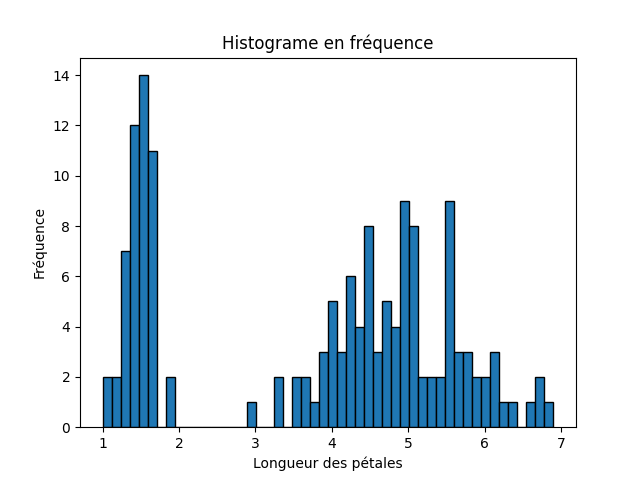
\includegraphics[width=1.1\textwidth]{img/Figure_3.png}
            \caption{\label{fig:histogramme_freq-petalLength}histogramme en fréquences de la variable petalLength}  
    \end{center}
    \end{minipage}\hfill
    \begin{minipage}{.48\linewidth}
        \begin{center}
            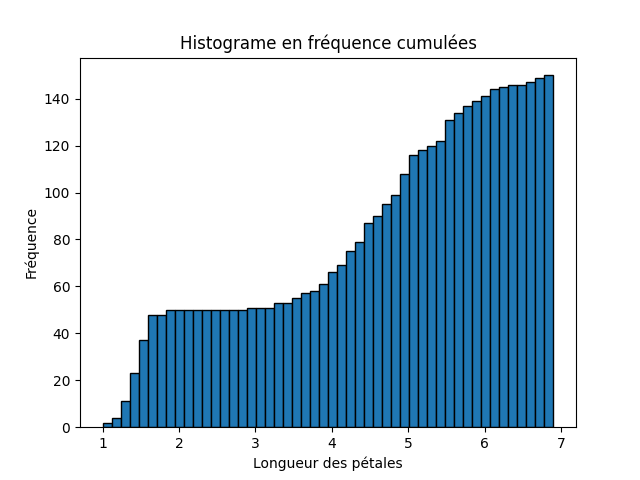
\includegraphics[width=1.1\textwidth]{img/Figure_4.png}
            \caption{\label{fig:histogramme_freq-petalLength-cumul}histogramme en fréquences cumulées de la variable petalLength}  
        \end{center}
    \end{minipage}
\end{figure}

\begin{lstlisting}[style=myPython, caption=Code python pour tracer les histogrammes, frame=lines]
n, x, _ = plt.hist(petallength, 50, edgecolor='black')
plt.title("Histograme en fréquence")
plt.show()

n_cumul, _, _ = plt.hist(petallength, 50, cumulative=True, edgecolor='black')
plt.title("Histograme en fréquence cumulées")
plt.show()
\end{lstlisting}

\vspace{.5cm}


\noindent
\textbf{Question~8~:} Décrire les caractéristiques de l’histogramme et analyser ces caractéristiques en fonction du nombre de classes.
\vspace{.3cm}

On remarque sur l'histogramme en fréquence qu'une majorité des longueurs de pétale est située entre 1 et 2~cm. Si l'on tient compte du nombre de classes, alors on peut penser à deux cas différents~: 
\begin{enumerate}
    \item Le premier serait que deux des trois classes ont majoritairement une longueur de pétale qui varie entre 1 et 2~cm. Dans ce cas, la troisième espèce a une longueur de pétale qui varie entre 3 et 7~cm.
    \item Le second cas serait qu'une des espèces a une longueur de pétale qui varie beaucoup moins que les deux autres. Par exemple l'espèce~1 varie entre 1 et 2~cm, tandis que l'espèce~2 et 3 varie entre 3 et 7~cm. Si l'on suit une 
          logique de probabilité, il est donc évident que l'effectif des longueurs de pétale entre 1 et 2~cm soit plus important puisqu’il y a le même nombre d'effectifs dans chaque espèce et que l'intervalle est plus faible.
\end{enumerate}

\vspace{.2cm}

Le cas numéro~2 semble le plus évident. Si l’on regarde l'histogramme en fréquence cumulé, on constate que le nombre d'effectifs augmente de 2/3 quand le pétale mesure entre 4 et 7~cm.\\
Grâce à l'histogramme en fréquences et l'histogramme en fréquences cumulées on peut conclure qu'une des espèces à une longueur de pétale plus petite que les deux autres, mais qui varie également beaucoup moins


\clearpage

\noindent
\textbf{Question~9~:} Tracer la boite à moustaches (boxplot) et rappeler les différents éléments la constituant.

\begin{figure}[!h]
    \begin{center}
        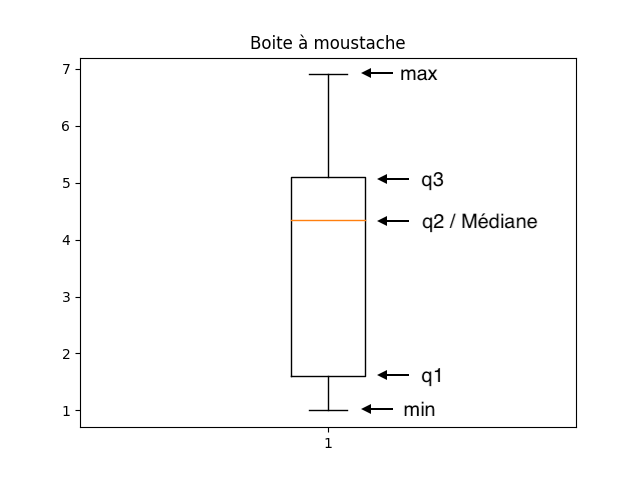
\includegraphics[width=.6\textwidth]{img/Figure_5.png}
        \caption{\label{fig:boite_moustache}Boite à moustache de la variable petalLength}  
    \end{center}
\end{figure}


\begin{lstlisting}[style=myPython, caption=Code Python pour tracer la boite à moustache, frame=lines]
plt.boxplot(petallength)
plt.title("Boite à moustache")
plt.show()
\end{lstlisting}

\vspace{.5cm}




\subsubsection*{Deuxième approche~: résumés numériques}
\vspace{.2cm}

\noindent
\textbf{Question~10~:} Calculer les résumés numériques de localisation (moyenne et médiane) et ceux de dispersion~: (écart-type, variance et quartiles). Retrouver en particulier, les valeurs des éléments de la boite à moustache.
\vspace{.2cm}


\begin{enumerate}
    \item \textbf{Formules utilisées~:}
        \begin{figure}[!h]
            \centering
            \begin{minipage}{.49\linewidth}
                \begin{itemize}
                    \item[--] Moyenne~: 
                        \begin{equation}
                            xn = \frac{1}{n} \sum_{i=0} ni.xi
                        \end{equation}

                    \item[--] Variance~: 
                        \begin{equation}
                            s^2_{n-1} = \frac{1}{n-1} \sum_{i=0} ni(xi - xn)^2
                        \end{equation}
                \end{itemize}
            \end{minipage}\hfill\vline
            \begin{minipage}{.49\linewidth}
                \begin{itemize}
                    \item[--] Médian~:
                        \begin{equation}
                            m=\text{valeur de } x \text{ à la position } \frac{n_{cumul}}{2}
                        \end{equation}

                    \item[--] Écart-type~:
                        \begin{equation}
                            s_{n-1} = \sqrt{s^2_{n-1}}
                        \end{equation}
                \end{itemize}
            \end{minipage}
        \end{figure}

        \begin{itemize}
            \item[--] Quartiles~:
                \begin{gather}
                        q1 = \text{valeur de } x \text{ à la position } \frac{n_{cumul}}{4} \\
                        q2 = m \\
                        q3 = \text{valeur de } x \text{ à la position } \frac{3*n_{cumul}}{4} 
                \end{gather}   
        \end{itemize}

        \clearpage

    \item \textbf{Valeurs obtenues~:}
    
        \vspace{.2cm}

        \begin{center}
            \begin{tabular}{| c |  c | c |}
                \hline
                \multirow{ 2}{*}{\textbf{Résumés numériques de localisation}} & moyenne & 3.701 \\ \cline{2-3}
                                                                    & médian  & 4.186 \\ \hline
                \multirow{ 5}{*}{\textbf{Résumés numériques de dispersion}}   & écart-type & 1.756 \\ \cline{2-3}
                                                                    & variance  & 3.084 \\ \cline{2-3}
                                                                    & q1  & 1.472 \\ \cline{2-3}
                                                                    & q2  & 4.186 \\ \cline{2-3}
                                                                    & q3  & 4.894 \\ \hline
            \end{tabular}
        \end{center}

        \vspace{.5cm}

    \item \textbf{Valeurs reportées sur les graphiques~:}
            \begin{figure}[!h]
                \centering
                \begin{minipage}{.48\linewidth}
                    \begin{center}
                        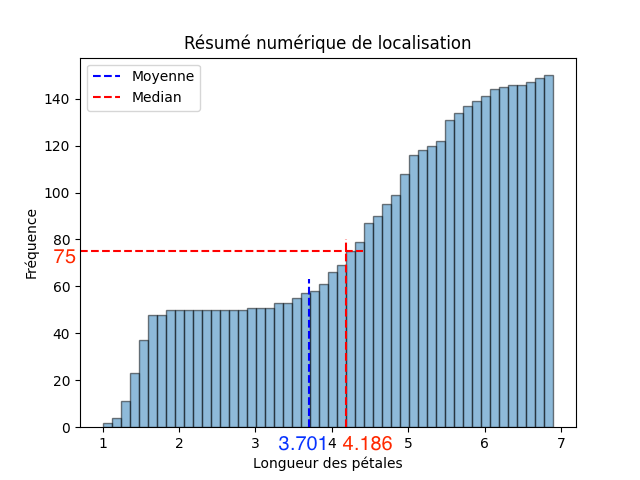
\includegraphics[width=1.1\textwidth]{img/Figure_6.png}
                        \caption{\label{fig:histogramme_freq-petalLength}histogramme en fréquences de la variable petalLength}  
                    \end{center}
                \end{minipage}\hfill
                \begin{minipage}{.48\linewidth}
                    \begin{center}
                        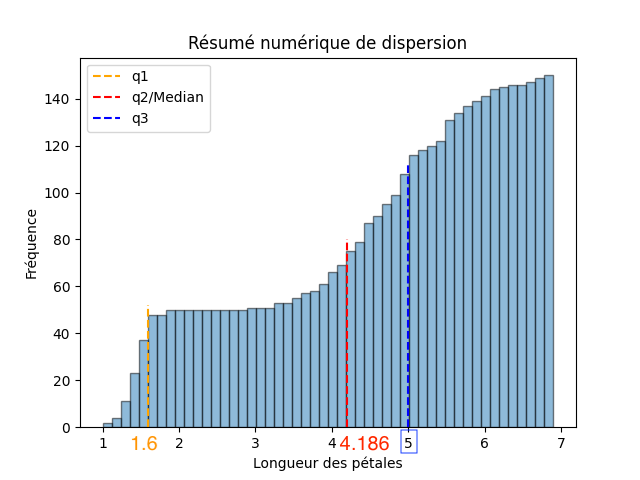
\includegraphics[width=1.1\textwidth]{img/Figure_7.png}
                        \caption{\label{fig:histogramme_freq-petalLength-cumul}histogramme en fréquences cumulées de la variable petalLength}  
                    \end{center}
                \end{minipage}
            \end{figure}
            
            \begin{figure}[!h]
                \begin{center}
                    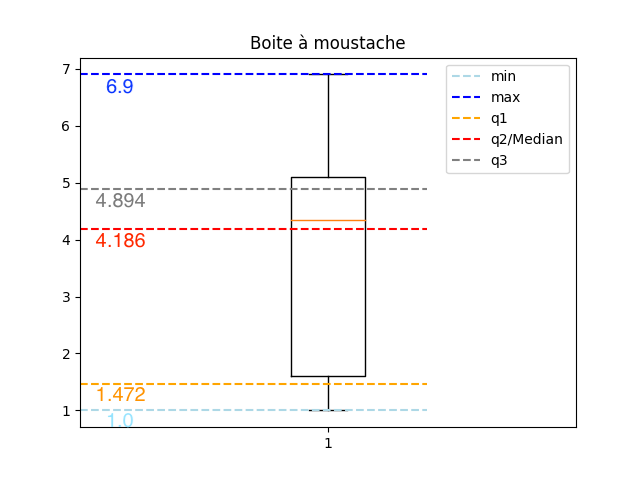
\includegraphics[width=.6\textwidth]{img/Figure_8.png}
                    \caption{\label{fig:boite_moustache}Boite à moustache de la variable petalLength}  
                \end{center}
            \end{figure}

            
    \clearpage


    \item \textbf{Code python~:}
    
    \vspace{.2cm}

    
\begin{lstlisting}[style=myPython, caption=Code python pour le résumé numérique, frame=lines]
def mean(n, x):
    n_max = len(df.values)
    res = 0
    for i in range(len(n)):
        res += (n[i] * x[i])
    ret = (1 / n_max) * res

    return round(ret, 3)

def median(n, x):
    n_median_index = np.where(n == (len(df.values) / 2))

    return float(x[n_median_index])

def variance(n, x, mean):
    n_max = len(df.values)
    res = 0
    for i in range(len(n)):
        res += n[i] * (x[i] - mean) ** 2
    ret = (1 / (n_max - 1)) * res

    return round(ret, 3)

def ecart_type(var):
    return round(np.sqrt(var), 3)

def quartiles(n, x):
    res = x[np.where(n < len(df.values) / 4)]
    q1 = res[-1]

    res = x[np.where(n < (3 * len(df.values)) / 4)]
    q3 = res[-1]

    q2 = median(n_cumul, x)

    return q1, q2, q3

print("RESUME NUMERIQUE DE LOCALISATION :")
print("Moyenne de petallenght:", mean(n, x))
print("Median de petallenght:", median(n_cumul, x), end="\n\n")

q1, q2, q3 = quartiles(n_cumul, x)
print("RESUME NUMERIQUE DE DISPERSION :")
print("Ecart-Type:", ecart_type(variance(n, x, mean(n, x))))
print("Variance:", variance(n, x, mean(n, x)))
print("Quartiles:", '\tq1 =', q1, '\tq2 =', q2, '\tq3 =', q3)
\end{lstlisting}

\begin{lstlisting}[style=myLog, caption=Résultat numérique du code python, frame=lines]
RESUME NUMERIQUE DE LOCALISATION :
Moyenne de petallenght: 3.701
Median de petallenght: 4.186

RESUME NUMERIQUE DE DISPERSION :
Ecart-Type: 1.756
Variance: 3.084
Quartiles: 	q1 = 1.472 	q2 = 4.186 	q3 = 4.894
\end{lstlisting}


\end{enumerate}






